\documentclass[xetex]{beamer}
\usepackage{polyglossia}
\setdefaultlanguage{english}
\usepackage{MnSymbol} % \powerset
\let\mathdollar\relax
\usepackage{fontspec}
\usepackage{xunicode}
\setsansfont{DejaVu Sans}
\setmonofont{DejaVu Sans Mono}
\usepackage{minted}
\usemintedstyle{colorful}
\newminted[coq]{coq}{
  frame=single, linenos, fontsize=\scriptsize
}
\usepackage{tikz}
\usetikzlibrary{arrows, shapes.multipart, calc}

\usetheme{Frankfurt}
\useoutertheme[subsection=false]{smoothbars}
\useinnertheme[shadow=true]{rounded}
\usecolortheme{orchid}
\usecolortheme{whale}
\setbeamertemplate{footline}[page number]

\newcommand{\newsection}[1]{
\section{#1}
\begin{frame}
  \frametitle{#1}
  \begin{center}
    {\Huge #1}
  \end{center}
\end{frame}
}

% Fix the counter
\usepackage{remreset}
\makeatletter
\@removefromreset{subsection}{section}
\makeatother
\stepcounter{subsection}

\title{Conception, mise en œuvre et vérification d'une analyse d'alias pour
CompCert, un compilateur C formellement vérifié}
\author{Valentin Robert}
\institute{INRIA Paris-Rocquencourt}
\date{15 décembre 2011}

\begin{document}

%%%%%%%%%%%%%%%%%%%%%%%%%%%%%%%%%%%%%%%%%%%%%%%%%%%%%%%%%%%%%%%%%%%%%%%%%%%%%%%

\setbeamertemplate{background canvas}{%
\tikz[remember picture,overlay] {
\node at (3, -6) {
\includegraphics[height=3cm] {enseirb.jpg}};
\node at (10, -6) {
\includegraphics[width=3cm] {inria.jpg}};
}}

\begin{frame}

\centering

\titlepage

Maître de stage~: Xavier Leroy

Tuteur~: Denis Barthou

\end{frame}

\setbeamertemplate{background canvas}{}

%%%%%%%%%%%%%%%%%%%%%%%%%%%%%%%%%%%%%%%%%%%%%%%%%%%%%%%%%%%%%%%%%%%%%%%%%%%%%%%

\begin{frame}
\tableofcontents
\end{frame}

%%%%%%%%%%%%%%%%%%%%%%%%%%%%%%%%%%%%%%%%%%%%%%%%%%%%%%%%%%%%%%%%%%%%%%%%%%%%%%%

\newsection{Contexte}

\begin{frame}[fragile]
\frametitle{Pourquoi vérifier formellement ?}

\tikzstyle{box}=[draw, rounded corners, very thick,
bottom color=white, top color=white!50!cyan]
\tikzstyle{arr}=[draw, -triangle 45]

\centering
\resizebox{\textwidth}{!}{
\begin{tikzpicture}[every text node part/.style={align=center}]

\visible<1->{
\node (spec) [box] at (0, 4) {Spécifications};
\node [green, right] at (spec.east) {✓};
\node (code) [box] at (0, 3) {Implémentation};
}

\visible<1-1>{
\node [red, right] at (code.east) {?};
}

\visible<2->{
\node [green, right] at (code.east) {✓};
\node (check) [box] at (5, 3.5) {
Model-checking\\
Analyses statiques
};
\path [arr] (spec) |- (check);
\path [arr] (code) |- (check);
}

\visible<3->{
\node (exec) [box] at (0, 1) {Exécutable};
\path [arr] (code) -- (exec)
  node [midway, right] {Compilation};
}

\visible<3-3>{
\node [red, below] at (exec.south) {?};
}

\visible<4->{
\node (test) [box] at (5, 1) {Tests, tests, tests...};
\path [arr] (exec) -- (test);
\node [green, below] at (exec.south) {?};
\node [green, right] at (test.east) {?};
}

\end{tikzpicture}
}

\end{frame}

%%%%%%%%%%%%%%%%%%%%%%%%%%%%%%%%%%%%%%%%%%%%%%%%%%%%%%%%%%%%%%%%%%%%%%%%%%%%%%%

\begin{frame}

\frametitle{CompCert}

\begin{figure}[H]
\begin{columns}
\begin{column}{0.4\textwidth}
\centering

\includegraphics[width=4cm]{k_and_r.png}
\end{column}
\begin{column}{0.2\textwidth}
\centering \resizebox{2cm}{!}{+}
\end{column}
\begin{column}{0.4\textwidth}
\centering

\includegraphics[width=3cm]{coq.png}
\end{column}
\end{columns}
\end{figure}

\end{frame}

%%%%%%%%%%%%%%%%%%%%%%%%%%%%%%%%%%%%%%%%%%%%%%%%%%%%%%%%%%%%%%%%%%%%%%%%%%%%%%%

\begin{frame}[fragile]

\frametitle{Impact réel ?}

Xuejun Yang, Yang Chen, Eric Eide, and John Regehr.
Finding and understanding bugs in c compilers.
\cite{Yang11}

\begin{itemize}

\item «reported more than 325 previously unknown bugs»

\item «Every compiler we tested was found to crash and also to silently
generate wrong code when presented with valid input.»

\item «The striking thing about our CompCert results is that the middleend bugs
we found in all other compilers are absent.»

\end{itemize}

\end{frame}

%%%%%%%%%%%%%%%%%%%%%%%%%%%%%%%%%%%%%%%%%%%%%%%%%%%%%%%%%%%%%%%%%%%%%%%%%%%%%%%

\begin{frame}[fragile]

\frametitle{Passes de CompCert}

\begin{figure}[H]
\centering
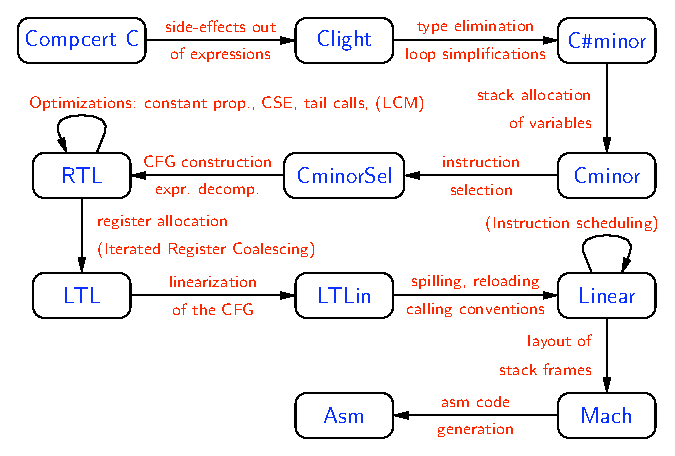
\includegraphics[height=6cm]{passes.eps}
\end{figure}

\end{frame}

%%%%%%%%%%%%%%%%%%%%%%%%%%%%%%%%%%%%%%%%%%%%%%%%%%%%%%%%%%%%%%%%%%%%%%%%%%%%%%%

\begin{frame}[fragile]

\frametitle{Analyse d'alias}

\begin{minted}[frame=single, linenos, fontsize=\footnotesize]{c}
int main() {
  int a, b, s0, s4, s8, *px, *py, *pz;
  px = &s0; py = &s4; pz = &s8;
  s8 = 42;
  a = 2 * s0 + 23;
  *py = 0;
  b = 2 * s0 + s8;
  return b;
}
\end{minted}


Ligne 7~:

\begin{itemize}

\pause

\item \mint{c}$2 * s0$ est-il le même qu'à la ligne 5 ?

\pause

\item \mint{c}$s8 == 42$ ?

\end{itemize}

\end{frame}

%%%%%%%%%%%%%%%%%%%%%%%%%%%%%%%%%%%%%%%%%%%%%%%%%%%%%%%%%%%%%%%%%%%%%%%%%%%%%%%

\begin{frame}[fragile]

\frametitle{Méthodologie}

\begin{itemize}

\item État de l'art

\pause

\item Prototype en OCaml

\pause

\item Traduction OCaml $\rightarrow$ Coq

\pause

\item Formalisation des propriétés attendues

\pause

\item Preuve de conformité de l'implémentation

\end{itemize}

\end{frame}

%%%%%%%%%%%%%%%%%%%%%%%%%%%%%%%%%%%%%%%%%%%%%%%%%%%%%%%%%%%%%%%%%%%%%%%%%%%%%%%

\newsection{Solution}

\begin{frame}[fragile]

\frametitle{Solution optimiste}

\centering

\tikzstyle{instr}=[draw, very thick]
\tikzstyle{arr}=[draw, -triangle 45, rounded corners]
\tikzstyle{reg}=[draw, minimum size=1cm]
\tikzstyle{mem}=[draw, minimum size=1cm]
\tikzstyle{lbl}=[draw, fill=white]
\tikzstyle{dot}=[draw, dotted]

\resizebox{!}{0.8\textheight}{
\begin{tikzpicture}
\node (entry)   [instr] at (0, 6)   {};
\node (iop1)    [instr] at (0, 4.5) {Iop};
\node (iop2)    [instr] at (0, 3)   {Iop};
\node (istore)  [instr] at (0, 1.5) {Istore};
\node (ireturn) [instr] at (0, 0)   {Ireturn};
\path [arr] (entry)     -- node [right, text width=0.5cm] (t1) {} (iop1);
\path [arr] (iop1)      -- node [right, text width=0.5cm] (t2) {} (iop2);
\path [arr] (iop2)      -- node [right, text width=0.5cm] (t3) {} (istore);
\path [arr] (istore)    -- node [right, text width=0.5cm] (t4) {} (ireturn);

\visible<2->{
\node (r1) [reg] at (3, 5) {R1};
\node (r2) [reg] at (3, 4) {R2};
\node (r3) [reg] at (3, 3) {R3};
\node (r4) [reg] at (3, 2) {R4};
\node (r5) [reg] at (3, 1) {R5};
\node (r6) [reg] at (3, 0) {R6};

\node (m1) [mem] at (6, 7) {0};
\node (m2) [mem] at (6, 6) {1};
\node (m3) [mem] at (6, 5) {...};
\node [lbl] at (m1.north) {b0};

\node (m4) [mem] at (6, 3) {0};
\node (m5) [mem] at (6, 2) {1};
\node (m6) [mem] at (6, 1) {...};
\node [lbl] at (m4.north) {b1};

\node (m7) [mem] at (6, -1) {0};
\node (m8) [mem] at (6, -2) {1};
\node (m9) [mem] at (6, -3) {...};
\node [lbl] at (m7.north) {b2};

\node [right] (s1) at (t1) {i1 = ⊥};
\path [dot] (r1.north west) -- (m1.north west);
\path [dot] (r6.south west) -- (m9.south west);
}

\visible<2>{
\path [dot] (s1.east) -- (r1.north west);
\path [dot] (s1.east) -- (r6.south west);
}

\visible<3->{
\node (s2) at (t2) {i2};
\path [arr] (r1.east) -- (m2.west);
}

\visible<3>{
\node [anchor=east] at (iop1.west) {"R1 peut pointer vers (b0, 1)"};
\path [dot] (s2.east) -- (r1.north west);
\path [dot] (s2.east) -- (r6.south west);
}

\visible<4->{
\node (s3) at (t3) {i3};
\path [arr] (r4.east) -- (m4.west);
\path [arr] (r4.east) -- (m5.west);
\path [arr] (r4.east) -- (m6.west);
}

\visible<4>{
\node [anchor=east] at (iop2.west) {"R4 peut pointer vers (b1, ?)"};
\path [dot] (s3.east) -- (r1.north west);
\path [dot] (s3.east) -- (r6.south west);
}

\visible<5->{
\node (s4) at (t4) {i4};
\path [arr] (m4.east) -| (9, 0) |- (m7.east);
\path [arr] (m4.east) -| (9, 0) |- (m8.east);
\path [arr] (m4.east) -| (9, 0) |- (m9.east);
\path [arr] (m5.east) -| (8, 0) |- (m7.east);
\path [arr] (m5.east) -| (8, 0) |- (m8.east);
\path [arr] (m5.east) -| (8, 0) |- (m9.east);
\path [arr] (m6.east) -| (7, 0) |- (m7.east);
\path [arr] (m6.east) -| (7, 0) |- (m8.east);
\path [arr] (m6.east) -| (7, 0) |- (m9.east);
}

\visible<5>{
\node [anchor=east] at (istore.west) {"(b1, ?) peut pointer vers (b2, ?)"};
\path [dot] (s4.east) -- (r1.north west);
\path [dot] (s4.east) -- (r6.south west);
}

\end{tikzpicture}
}

\end{frame}

%%%%%%%%%%%%%%%%%%%%%%%%%%%%%%%%%%%%%%%%%%%%%%%%%%%%%%%%%%%%%%%%%%%%%%%%%%%%%%%

\tikzstyle{box}=[]
\tikzstyle{edge}=[draw, very thick]
\newsavebox{\hierarchy}
\savebox{\hierarchy}{
\begin{tikzpicture}[every text node part/.style={align=center}, scale=2]

\node [box] (all) at (8, 3) {All};

\node [box] (allocs)    at ( 2, 2) {Allocs};
\node [box] (stack)     at ( 6, 2) {Stack};
\node [box] (other)     at (10, 2) {Other};
\node [box] (globals)   at (14, 2) {Globals};

\node [box] (alloc1)    at ( 1, 1) {Alloc 1};
\node [box] (allocx)    at ( 2, 1) {...};
\node [box] (alloca)    at ( 3, 1) {Alloc a};
\node at (alloca.south) {...};
\node [box] (global1)   at (13, 1) {Global 1};
\node [box] (globalx)   at (14, 1) {...};
\node [box] (globalg)   at (15, 1) {Global g};
\node at (globalg.south) {...};

\node [box] (stack0)    at ( 5, 1) {(Stack, 0)};
\node [box] (stackx)    at ( 6, 1) {...};
\node [box] (stacki)    at ( 7, 1) {(Stack, i)};
\node [box] (other0)    at ( 9, 1) {(Other, 0)};
\node [box] (otherx)    at (10, 1) {...};
\node [box] (otheri)    at (11, 1) {(Other, i)};

\node [box] (alloc10)   at ( 0, 0) {(Alloc 1, 0)};
\node [box] (alloc1x)   at ( 1, 0) {...};
\node [box] (alloc1i)   at ( 2, 0) {(Alloc 1, i)};
\node [box] (global10)  at (12, 0) {(Global 1, 0)};
\node [box] (global1x)  at (13, 0) {...};
\node [box] (global1i)  at (14, 0) {(Global 1, i)};

\path [edge] (all) -- (allocs);
\path [edge] (all) -- (stack);
\path [edge] (all) -- (other);
\path [edge] (all) -- (globals);

\path [edge] (allocs) -- (alloc1);
\path [edge] (allocs) -- (allocx);
\path [edge] (allocs) -- (alloca);
\path [edge] (globals) -- (global1);
\path [edge] (globals) -- (globalx);
\path [edge] (globals) -- (globalg);

\path [edge] (stack) -- (stack0);
\path [edge] (stack) -- (stackx);
\path [edge] (stack) -- (stacki);
\path [edge] (other) -- (other0);
\path [edge] (other) -- (otherx);
\path [edge] (other) -- (otheri);

\path [edge] (alloc1) -- (alloc10);
\path [edge] (alloc1) -- (alloc1x);
\path [edge] (alloc1) -- (alloc1i);
\path [edge] (global1) -- (global10);
\path [edge] (global1) -- (global1x);
\path [edge] (global1) -- (global1i);

\end{tikzpicture}
}

%%%%%%%%%%%%%%%%%%%%%%%%%%%%%%%%%%%%%%%%%%%%%%%%%%%%%%%%%%%%%%%%%%%%%%%%%%%%%%%

\begin{frame}[fragile]
\frametitle{Domaine de l'analyse}

\newcommand\tB{\mathcal{B}}
\newcommand\tL{\mathcal{L}}
\newcommand\tS{\mathcal{S}}
\newcommand\tR{\mathcal{R}}
\newcommand\tM{\mathcal{M}}

$\tR$ : ensemble des registres de la fonction

$
\only<1>{\tB}
\only<2->{\textcolor{blue}{\bar{\tB}}}
$ : ensemble des blocs
\only<2->{\textcolor{blue}{abstraits}}
\only<3->{\textcolor{blue}{hiérarchisés}}

$
\only<1>{\tL}
\only<2->{\textcolor{blue}{\bar{\tL}}}
= \{(b, o) | b \in
\only<1>{\tB}
\only<2->{\textcolor{blue}{\bar{\tB}}}
, o \in \mathit{range(int)}\}$

$
\only<1>{\tS}
\only<2->{\textcolor{blue}{\bar{\tS}}}
= \powerset{(
\only<1>{\tL}
\only<2->{\textcolor{blue}{\bar{\tL}}}
\only<3->{\cup \textcolor{blue}{\bar{\tB}}}
)}$

\begin{block}{Domaine}
$(\tR \rightarrow
\only<1>{\tS}
\only<2->{\textcolor{blue}{\bar{\tS}}}
,
\only<3>{(}
\only<1>{\tL}
\only<2->{\textcolor{blue}{\bar{\tL}}}
\only<3>{\cup \textcolor{blue}{\bar{\tB}})}
\leadsto
\only<1>{\tS}
\only<2->{\textcolor{blue}{\bar{\tS}}}
)$
\end{block}

\visible<3->{
\resizebox{\textwidth}{!}{\usebox{\hierarchy}}
}

\end{frame}

%%%%%%%%%%%%%%%%%%%%%%%%%%%%%%%%%%%%%%%%%%%%%%%%%%%%%%%%%%%%%%%%%%%%%%%%%%%%%%%

\begin{frame}[fragile]

\frametitle{Dictionnaire hiérarchique}

\resizebox{\textwidth}{!}{\usebox{\hierarchy}}

\begin{minted}
[frame=single, linenos, fontsize=\tiny]
{coq}
Module Type OMapInterface (O: OverlapInterface) (L: SEMILATTICE).
Parameter t: Type.
Parameter get: O.t -> t -> L.t.
Parameter add: O.t -> L.t -> t -> t.

Axiom get_add_same: forall k s m,   L.ge (get k (add k s m)) s.
Axiom get_add:      forall x y s m, L.ge (get x (add y s m)) (get x m).
Axiom get_add_over: forall x y s m,
  O.overlap x y ->
  L.ge (get x (add y s m)) s.
End OMapInterface.
\end{minted}

\end{frame}

%%%%%%%%%%%%%%%%%%%%%%%%%%%%%%%%%%%%%%%%%%%%%%%%%%%%%%%%%%%%%%%%%%%%%%%%%%%%%%%

\begin{frame}[fragile]

\frametitle{Algorithme de Kildall}

\centering

\begin{tikzpicture}[every text node part/.style={align=center}]

\tikzstyle{box}=[draw, very thick]
\tikzstyle{arr}=[draw, -triangle 45]

\node (entry)   [box] at (9, 6) {};
\node (iop)     [box] at (9, 4.5) {Iop};
\node (iload)   [box] at (9, 3) {Iload};
\node (icond)   [box] at (9, 1.5) {Icond};
\node (iop')    [box] at (8, 0) {Iop};
\node (ireturn) [box] at (10, 0) {Ireturn};
\path [arr] (entry) -- node [right, text width=0.5cm] (s1) {} (iop);
\path [arr] (iop)   -- node [right, text width=0.5cm] (s2) {} (iload);
\path [arr] (iload) -- node [right, text width=0.5cm] (s3) {} (icond);
\path [arr] (icond) -- node [left,  text width=0.5cm] (s4) {} (iop');
\path [arr] (icond) -- node [right, text width=0.5cm] (s5) {} (ireturn);
\path [arr] (iop'.south)
    -- ++(0, -0.2)
    -- ++(-1, 0)
    -- node [left, text width=0.5cm] (s6) {} ($ (iload.center) - (2, 0) $)
    -- (iload.west)
;

\tikzstyle{state}=
[shape=circle,draw=blue!50,fill=blue!20,text width=0.6cm, text centered]
\tikzstyle{edge}=[draw, -triangle 45, dotted]
\tikzstyle{mainstate}=[state, very thick, draw=black]
\tikzstyle{mainedge}=[draw, -triangle 45, very thick]

\visible<2->{
\node (bot) [state] at (3, 0) {$\bot$};
\node (a)   [state] at (1, 2) {$a$};
\node (b)   [state] at (3, 2) {$b$};
\node (c)   [state] at (5, 2) {$c$};
\node (ab)  [state] at (1, 4) {$ab$};
\node (ac)  [state] at (3, 4) {$ac$};
\node (bc)  [state] at (5, 4) {$bc$};
\node (top) [state] at (3, 6) {$\top$};
\path [edge]        (bot)   -- (a);
\path [edge]        (bot)   -- (c);
\path [edge]        (a)     -- (ab);
\path [edge]        (a)     -- (ac);
\path [edge]        (b)     -- (bc);
\path [edge]        (c)     -- (ac);
\path [edge]        (c)     -- (bc);
\path [edge]        (ab)    -- (top);
\path [edge]        (bc)    -- (top);
\path [edge]        (ac)    -- (top);

\path [draw, dotted] (bc.east) -- (s6.north west);
\path [draw, dotted] (bot.south east) -- (s6.south west);
}

\visible<2>{
\node at (s1) {$a$};
\node at (s2) {$\bot$};
\node at (s3) {$\bot$};
\node at (s4) {$\bot$};
\node at (s5) {$\bot$};
\node at (s6) {$\bot$};
\node [mainstate] at (bot) {$\bot$};
\path [edge] (bot) -- (b);
}
\visible<2-5>{
\path [edge] (b) -- (ab);
}
\visible<3->{
\node [red] at (s1) {$a$};
\path [mainedge] (bot) -- (b);
}
\visible<3>{
\node [green] at (s2) {$a$};
\node [red] at (s3) {$\bot$};
\node [red] at (s4) {$\bot$};
\node [red] at (s5) {$\bot$};
\node [green] at (s6) {$b$};
}
\visible<3-5>{
\node [mainstate] at (b) {$b$};
}
\visible<4->{
\node [red] at (s2) {$a$};
}
\visible<4>{
\node [green] at (s3) {$ab$};
\node [red] at (s4) {$\bot$};
\node [red] at (s5) {$\bot$};
\node [red] at (s6) {$b$};
}
\visible<5->{
\node [red] at (s3) {$ab$};
}
\visible<5>{
\node [green] at (s4) {$ab$};
\node [green] at (s5) {$ab$};
\node [red] at (s6) {$b$};
}
\visible<6->{
\node [red] at (s4) {$ab$};
\node [red] at (s5) {$ab$};
\node [green] at (s6) {$ab$};
\path [mainedge] (b) -- (ab);
\node [mainstate] at (ab) {$ab$};
}
\visible<7->{
\node [red] at (s6) {$ab$};
}

\end{tikzpicture}

\end{frame}

%%%%%%%%%%%%%%%%%%%%%%%%%%%%%%%%%%%%%%%%%%%%%%%%%%%%%%%%%%%%%%%%%%%%%%%%%%%%%%%

\newsection{Preuve}

\begin{frame}[fragile]

\frametitle{Interprétation abstraite}

\tikzstyle{box}=[draw, minimum size=1cm]
\tikzstyle{arr}=[draw, very thick, -triangle 45]
\tikzstyle{abs}=[draw, very thick, green]
\tikzstyle{code}=[anchor=west, minimum size=8.8cm, text width=8.6cm]
\centering
\resizebox{\textwidth}{!}{
\begin{tikzpicture}

% Code
\node (c5) [code] at (10, 3)    {5: R1 := \&stack(0)};
\node (c4) [code] at (10, 2.5)  {4: R2 := \&global1 + R3};
\node (c3) [code] at (10, 2)    {3: R6 = malloc(2);};
\node (c2) [code] at (10, 1.5)  {2: if (...) goto 3 else goto 1;};
\node (c1) [code] at (10, 1)    {1: return R2};
\visible<1>{\node at (c5.west) {▶};}
\visible<2>{\node at (c4.west) {▶};}
\visible<3>{\node at (c3.west) {▶};}
\visible<4>{\node at (c2.west) {▶};}
\visible<5>{\node at (c3.west) {▶};}
\visible<6>{\node at (c2.west) {▶};}
\visible<7>{\node at (c1.west) {▶};}

% Text
\node [red]     at (  2,  13)   {Exécution};
\node [blue]    at ( 15,  13)   {Analyse};
\node [green]   at (8.5,  13)    {Abstraction};

% Actual registers
\node (r1) [box] at ( 2, 10) {R1};
\node (r2) [box] at ( 2,  9) {R2};
\node (r3) [box] at ( 2,  8) {R3};
\node (r4) [box] at ( 2,  7) {R4};
\node (r5) [box] at ( 2,  6) {R5};
\node (r6) [box] at ( 2,  5) {R6};

% Actual memory
\node (m1) [box] at ( 6, 12) {};
\node (m2) [box] at ( 6, 11) {};
\node (m3) [box] at ( 6,  9) {};
\node (m4) [box] at ( 6,  8) {};
\visible<4->{
\node (m5) [box] at ( 6,  6) {};
\node (m6) [box] at ( 6,  5) {};
}
\visible<6->{
\node (m7) [box] at ( 6,  3) {};
\node (m8) [box] at ( 6,  2) {};
}

% Abstract memory
\node (am1) [box] at (11, 12) {};
\node (am2) [box] at (11, 11) {};
\node (am3) [box] at (11,  9) {};
\node (am4) [box] at (11,  8) {};
\visible<4->{
\node (am5) [box] at (11,  6) {};
\node (am6) [box] at (11,  5) {};
}

% Abstract registers
\node (ar1) [box] at (15, 10) {R1};
\node (ar2) [box] at (15,  9) {R2};
\node (ar3) [box] at (15,  8) {R3};
\node (ar4) [box] at (15,  7) {R4};
\node (ar5) [box] at (15,  6) {R5};
\node (ar6) [box] at (15,  5) {R6};

% Legend
\node [above] at (m1.north)   {blocs concrets};
\node [above] at (am1.north)  {blocs abstraits};

% Abstracter
\node at (8.5, 11.5) {Stack};
\path [abs] (m1.north east)  -- (am1.north west);
\path [abs] (m2.south east)  -- (am2.south west);
\node at (8.5, 8.5) {Global 1};
\path [abs] (m3.north east)  -- (am3.north west);
\path [abs] (m4.south east)  -- (am4.south west);
\visible<4->{
\node at (8.5, 5.5) {Alloc 3};
\path [abs] (m5.north east)  -- (am5.north west);
\path [abs] (m6.south east)  -- (am6.south west);
}
\visible<6->{
\node at (8.5, 4) {Alloc 3};
\path [abs] (m7.north east)  -- (am5.north west);
\path [abs] (m8.south east)  -- (am6.south west);
}

% Olea (Stack, 0) R1
\visible<2->{
\path [arr, red]    (r1.east)   -- (m1.west);
\path [arr, blue]   (ar1.west)  -- (am1.east);
}
% Olea (Global 1, *(R1)) R2
\visible<3->{
\path [arr, red]    (r2.east)   -- (m3.west);
\path [arr, blue]   (ar2.west)  -- (am3.east);
\path [arr, blue]   (ar2.west)  -- (am4.east);
}
% Malloc 2 R6
\visible<4-5>{
\path [arr, red]    (r6.east)   -- (m5.west);
}
\visible<4->{
\path [arr, blue]   (ar6.west)  -- (am5.east);
}
% Malloc 2 R6
\visible<6->{
\path [arr, red]    (r6.east)   -- (m7.west);
}
\visible<6->{
\path [arr, blue]   (ar6.west)  -- (am5.east);
}

\end{tikzpicture}
}

\end{frame}

%%%%%%%%%%%%%%%%%%%%%%%%%%%%%%%%%%%%%%%%%%%%%%%%%%%%%%%%%%%%%%%%%%%%%%%%%%%%%%%

\begin{frame}[fragile]

\frametitle{Invariants de preuve (1)}

\begin{coq}
Definition valsat (v: val) (abs: abstracter) (s: ptset) :=
match v with
| Vptr b o =>
  match abs b with
  | Some ab => PTS.In (ab, o) s
  | None    => PTS.eq s PTS.top
  end
| _        => True
end.
\end{coq}

\pause

\begin{minted}
[firstnumber=10, frame=single, linenos, fontsize=\scriptsize]
{coq}
Definition regsat (r: reg) (rs: regset) abs (ptm: ptmap) :=
valsat rs#r abs (mpt (Reg r) ptm).
\end{minted}

\pause

\begin{minted}
[firstnumber=12, frame=single, linenos, fontsize=\scriptsize]
{coq}
Definition memsat
(b: block) (o: offset) (m: mem) abs (ptm: ptmap) := forall v
  (LOAD: Mem.loadv Mint32 m (Vptr b o) = Some v)
  ,
  (match abs b with
    | Some ab => valsat v abs (mpt (Loc (ab, o)) ptm)
    | None    => False
    end).
\end{minted}

\end{frame}

%%%%%%%%%%%%%%%%%%%%%%%%%%%%%%%%%%%%%%%%%%%%%%%%%%%%%%%%%%%%%%%%%%%%%%%%%%%%%%%

\begin{frame}[fragile]

\frametitle{Invariants de preuve (2)}

\begin{minted}
[frame=single, linenos, fontsize=\tiny]
{coq}
Inductive satisfy (ge: genv) (ptmm: result) (abs: abstracter): state -> Prop :=
| satisfy_state: forall cs f bsp pc rs m ptm
  (STK:   ok_stack ge (Mem.nextblock m) cs)
  (MEM:   ok_abs_mem abs m)
  (GENV:  ok_abs_genv abs ge)
  (SP:    abs bsp = Some Stack)
  (RES:   funanalysis f = Some ptmm)
  (PTM:   ptm = ptmm#pc)
  (WF:    PTM.well_formed ptm)
  (RSAT:  forall r, regsat r rs abs ptm)
  (MSAT:  forall b o, memsat b o m abs ptm)
  ,
  satisfy ge ptmm abs (State cs f (Vptr bsp Int.zero) pc rs m)
| satisfy_callstate: forall cs f args m
  (MEM:   ok_abs_mem abs m)
  (STK:   ok_stack ge (Mem.nextblock m) cs)
  (GENV:  ok_abs_genv abs ge)
  ,
  satisfy ge ptmm abs (Callstate cs f args m)
| satisfy_returnstate: forall cs v m
  (MEM:   ok_abs_mem abs m)
  (STK:   ok_stack ge (Mem.nextblock m) cs)
  (GENV:  ok_abs_genv abs ge)
  ,
  satisfy ge ptmm abs (Returnstate cs v m)
.
\end{minted}

\end{frame}

%%%%%%%%%%%%%%%%%%%%%%%%%%%%%%%%%%%%%%%%%%%%%%%%%%%%%%%%%%%%%%%%%%%%%%%%%%%%%%%

\begin{frame}[fragile]

\frametitle{Théorèmes}

\begin{coq}
Theorem satisfy_init: forall p st
  (IS: initial_state p st)
  ,
  exists ptm, exists abs,
  satisfy (Genv.globalenv p) ptm abs st.
\end{coq}

\pause

\begin{coq}
Theorem satisfy_step: forall ge st t st' ptm abs
  (SAT:  satisfy ge ptm abs st)
  (STEP: step ge st t st')
  ,
  exists ptm', exists abs',
  satisfy ge ptm' abs' st'.
\end{coq}

\end{frame}

%%%%%%%%%%%%%%%%%%%%%%%%%%%%%%%%%%%%%%%%%%%%%%%%%%%%%%%%%%%%%%%%%%%%%%%%%%%%%%%

\newsection{Résultats}

\begin{frame}[fragile]

\frametitle{Résultats (1)}

\begin{minted}[frame=single, linenos, fontsize=\footnotesize]{c}
int main() {
  int a, b, s0, s4, s8, *px, *py, *pz;
  px = &s0; py = &s4; pz = &s8;
  s8 = 42;
  a = 2 * s0 + 23;
  *py = 0;
  b = 2 * s0 + s8;
  return b;
}
\end{minted}


\end{frame}

%%%%%%%%%%%%%%%%%%%%%%%%%%%%%%%%%%%%%%%%%%%%%%%%%%%%%%%%%%%%%%%%%%%%%%%%%%%%%%%

\begin{frame}[fragile]

\frametitle{Résultats (2)}

\begin{minted}
[frame=single, fontsize=\fontsize{6pt}{6pt}\selectfont]
{coq}
| Globals -> ⊤ | Other -> ⊤
14: Iop {op: Olea Ainstack 0} {args: []} {dest: R3} {succ: 13}
| Globals -> ⊤ | Other -> ⊤
| R3 -> ({}, {(Stack, 0)})
13: Iop {op: Olea Ainstack 4} {args: []} {dest: R2} {succ: 12}
| Globals -> ⊤ | Other -> ⊤
| R2 -> ({}, {(Stack, 4)}) | R3 -> ({}, {(Stack, 0)})
12: Iop {op: Olea Ainstack 8} {args: []} {dest: R1} {succ: 11}
| Globals -> ⊤ | Other -> ⊤
| R1 -> ({}, {(Stack, 8)}) | R2 -> ({}, {(Stack, 4)}) | R3 -> ({}, {(Stack, 0)})
11: Iop {op: Ointconst 42} {args: []} {dest: R14} {succ: 10}
| Globals -> ⊤ | Other -> ⊤
| R1 -> ({}, {(Stack, 8)}) | R2 -> ({}, {(Stack, 4)}) | R3 -> ({}, {(Stack, 0)})
10: Istore {chunk: Mint32} {addr: Ainstack 8} {args: []} {src: R14} {succ: 9}
| Globals -> ⊤ | Other -> ⊤
| R1 -> ({}, {(Stack, 8)}) | R2 -> ({}, {(Stack, 4)}) | R3 -> ({}, {(Stack, 0)})
9: Iload {chunk: Mint32} {addr: Ainstack 0} {args: []} {dest:R13} {succ: 8}
| Globals -> ⊤ | Other -> ⊤
| R1 -> ({}, {(Stack, 8)}) | R2 -> ({}, {(Stack, 4)}) | R3 -> ({}, {(Stack, 0)})
8: Iop {op: Olea Ascaled (2, 23)} {args: [R13]} {dest: R8} {succ: 7}
| Globals -> ⊤ | Other -> ⊤
| R1 -> ({}, {(Stack, 8)}) | R2 -> ({}, {(Stack, 4)}) | R3 -> ({}, {(Stack, 0)})
7: Iop {op: Ointconst 0} {args: []} {dest: R12} {succ: 6}
| Globals -> ⊤ | Other -> ⊤
| R1 -> ({}, {(Stack, 8)}) | R2 -> ({}, {(Stack, 4)}) | R3 -> ({}, {(Stack, 0)})
6: Istore {chunk: Mint32} {addr: Aindexed 0} {args: [R2]} {src: R12} {succ: 5}
| Globals -> ⊤ | Other -> ⊤
| R1 -> ({}, {(Stack, 8)}) | R2 -> ({}, {(Stack, 4)}) | R3 -> ({}, {(Stack, 0)})
[...]
\end{minted}

\end{frame}

%%%%%%%%%%%%%%%%%%%%%%%%%%%%%%%%%%%%%%%%%%%%%%%%%%%%%%%%%%%%%%%%%%%%%%%%%%%%%%%

\begin{frame}[fragile]

\frametitle{Performance de l'analyse}

\centering

\begin{table}[!h]
\resizebox{\textwidth}{!}{
\begin{tabular}{|l|c|c|}
\hline
Test (lignes de code)&
Compilation sans analyse (s)&
Compilation avec analyse (s)\\
\hline
chomp (370) & 0.080 & 0.115\\
aes (1453) & 0.160 & 0.448\\
raytracer (2560) & 1.713 & 2.723\\
compression (4788) & 0.985 & 1.215\\
spass (69073) & 16.906 & 56.693\\
\hline
\end{tabular}
}
\end{table}

\end{frame}

%%%%%%%%%%%%%%%%%%%%%%%%%%%%%%%%%%%%%%%%%%%%%%%%%%%%%%%%%%%%%%%%%%%%%%%%%%%%%%%

\newsection{Conclusion}

\begin{frame}[fragile]

\begin{itemize}

\item Yes we can! $\square$

\end{itemize}

\end{frame}

%%%%%%%%%%%%%%%%%%%%%%%%%%%%%%%%%%%%%%%%%%%%%%%%%%%%%%%%%%%%%%%%%%%%%%%%%%%%%%%

\begin{frame}[fragile]

\centering

{\Large Merci de votre attention.}

\end{frame}

%%%%%%%%%%%%%%%%%%%%%%%%%%%%%%%%%%%%%%%%%%%%%%%%%%%%%%%%%%%%%%%%%%%%%%%%%%%%%%%
\begin{frame}
\frametitle{Références}
\bibliographystyle{alpha}
\bibliography{biblio}
\end{frame}

\end{document}
